% load relevant packages
\documentclass[11pt,a4paper]{article}
\usepackage[hyperref]{acl2020}
\usepackage{booktabs}
\usepackage{xcolor}
\usepackage{makecell}
\usepackage{float}
\usepackage{tabularx}
\usepackage{times}
\usepackage{multirow}
\usepackage{lipsum}
\usepackage{amsmath}
\usepackage{amssymb}
\usepackage{mathtools}
\usepackage{latexsym}
\usepackage{graphicx}
\usepackage{microtype}
\usepackage{array}
\aclfinalcopy
%\setlength\titlebox{5cm}
\newcommand\BibTeX{B\textsc{ib}\TeX}
\renewcommand{\UrlFont}{\ttfamily\small}
\newcolumntype{P}[1]{>{\raggedright\arraybackslash}p{#1}}
\graphicspath{{../../img/}}

% administrative details
\title{Investigating the isometric behaviour of Neural Machine Translation models on binary semantic equivalence spaces}
\author{Atreya Shankar \\
  Cognitive Systems, University of Potsdam \\
  Department of Computational Linguistics, University of Zürich \\
  \texttt{atreya.shankar@\{uni-potsdam.de,uzh.ch\}}}
\date{\today}

% start document
\begin{document}

% produce title
\maketitle

% abstract
\begin{abstract}
In this research, we assume that well-performing Neural Machine Translation (NMT) models function approximately isometrically on semantic metric spaces and hypothesize that the frequency of such isometric behaviour correlates positively with general model performance. We conduct our investigation by using two NMT models of varying performance to translate semantically-equivalent German paraphrases, based off diverse WMT19 test data references, to English. We simplify the notion of semantic metric spaces into probabilistic binary semantic equivalence spaces and compute these using three transformer language models fine-tuned on Google's PAWS-X paraphrase detection task. By analyzing the paraphrase detection outputs, we show that the frequency of semantically isometric behaviour indeed correlates positively with general model performance. With our final results, we provide evidence both for and against claims made by other studies on automatic sequence evaluation metrics and NMT models' volatility towards adversarial paraphrases.
\end{abstract}

% body
\section{Introduction}

Isometry is defined mathematically as a distance-preserving transformation between two metric spaces \cite{coxeter1961introduction}. In this research, we view Neural Machine Translation (NMT) models from the perspective of semantic isometry and assume that well-performing NMT models function approximately isometrically on semantic metric spaces. That is to say, if two sentences are semantically equivalent on the source side, they should remain semantically equivalent after translation on the target side given a well-performing NMT model. A simplified illustration of isometry in higher dimensional functional spaces can be seen in Figure \ref{isometry_visual}. We hypothesize that the frequency of such semantically isometric behaviour correlates positively with general model performance. 

In order to conduct our investigation, we start by acquiring semantically equivalent German paraphrases of WMT19 legacy and additional test references from \citet{freitag-bleu-paraphrase-references-2020}. Next, we utilize two NMT models of varying performance, specifically the state-of-the-art (SOTA) Facebook AI Research's (FAIR) WMT19 winning single transformer \cite{ng2019facebook} and the non-SOTA Scaling NMT WMT16 Transformer \cite{ott2018scaling}, to translate the aforementioned paraphrases to English.

\begin{figure}
  \centering
  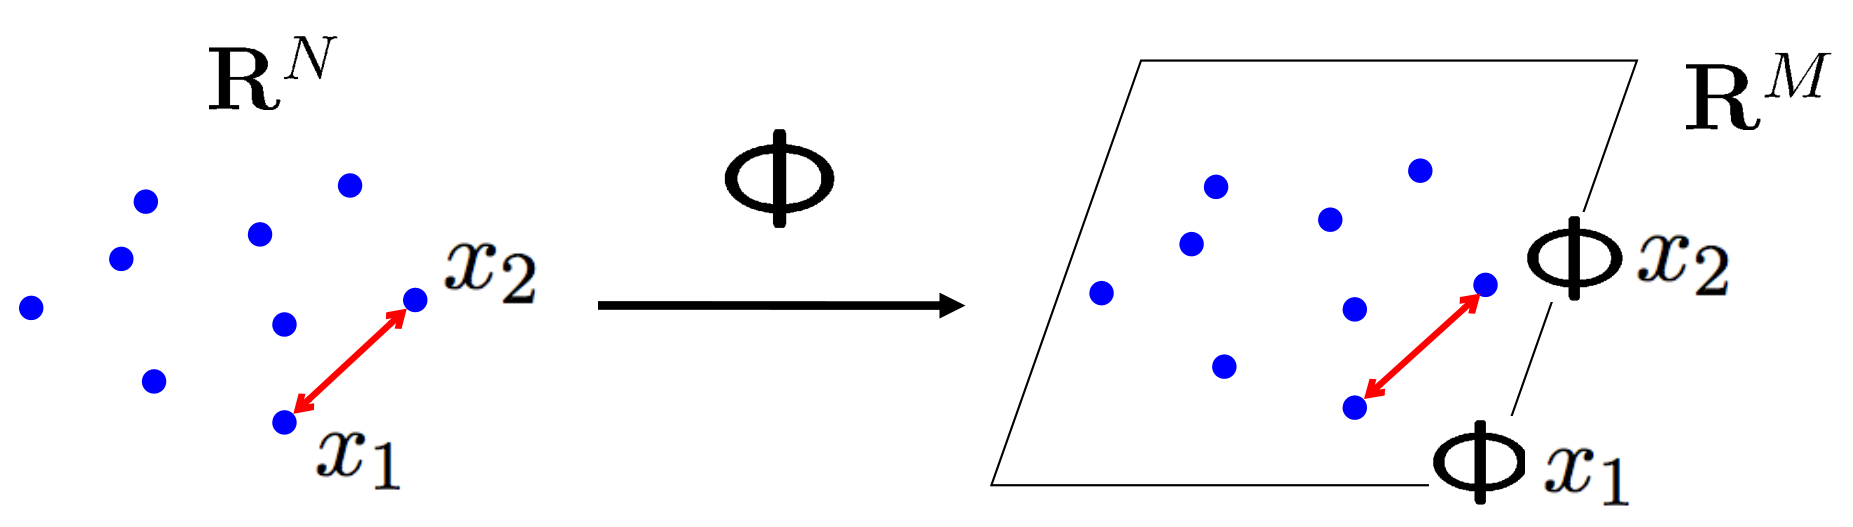
\includegraphics[trim={0cm 0cm 0cm 0cm},clip,width=0.52\textwidth]{isometry_visualized.png}
  \caption{Illustration of isometry in higher dimensional functional transformations \citep{Hegde-Numax}}
  \label{isometry_visual}
\end{figure}

Next, we simplify the notion of semantic metric spaces into probabilistic binary semantic equivalence spaces and utilize three well-performing paraphrase detection models to approximate these spaces in the NMT models' inputs and translations. These paraphrase detection models are based off the mBERT\textsubscript{Base} \cite{devlin-etal-2019-bert}, XLM-R\textsubscript{Base} \cite{conneau2019unsupervised} and XLM-R\textsubscript{Large} \cite{conneau2019unsupervised} pre-trained multilingual language models; which are correspondingly fine-tuned on Google's PAWS-X paraphrase detection task \cite{pawsx2019emnlp, hu2020xtreme}.
 
Using the outputs of the paraphrase detection models, we show that the frequency of semantically isometric behaviour correlates positively with general model performance. With our final results, we provide evidence both for and against claims made by other studies on automatic sequence evaluation metrics and NMT models' volatility towards adversarial paraphrases. We release our latest models and source code in our public GitHub repository\footnote{\url{https://github.com/atreyasha/semantic-isometry-nmt}}.

\section{Isometry and approximations}

Isometry in the context of NMT and semantic metric spaces can be exactly expressed as follows; where $s_i \in \mathbb{R}^{V \times N}$ refers to an input sentence's tokenized matrix form for vocabulary size $V$ and maximum sentence length $N$, $f: \mathbb{R}^{V \times N} \to \mathbb{R}^{V' \times N'}$ refers to the NMT model's inference function which translates sentences from language $X$ to $Y$ and $D_L: \mathbb{R}^{V \times 2N} \to \mathbb{R}_+$ refers to a semantic distance metric function for language $L$ corresponding to the language of the respective sentences:

\begin{equation}  
  \label{exact_isometry_eqn}
  D_X(s_1,s_2) = D_Y(f(s_1),f(s_2))
\end{equation}

While elegant, this representation of isometry is problematic for two key reasons.

\begin{enumerate}
\item Exact isometry may not be a practical condition given real-life data instances with stochastic noise.
\item Constructing continuous semantic metric spaces from discrete textual data is a difficult task and is in itself a developing field of research \cite{cer2017semeval, michel2019evaluation}.
\end{enumerate}

\subsection{Approximate isometry}

To address the first issue, we loosen the constraints of exact isometry to approximate isometry:

\begin{equation} 
  \label{approx_isometry_eqn}
  D_X(s_1,s_2) \approx D_Y(f(s_1),f(s_2)) 
\end{equation}

With this approximation, we can simplify the isometric relationship further into a binary semantic equivalence function $S_L: \mathbb{R}^{V \times 2N} \to \{0,1\}$, which compresses semantic distance metrics to semantic equivalence ($S_L=1$) and inequivalence ($S_L=0$) depending on some variable threshold $\delta_L \in \mathbb{R}_+$:

\begin{equation}
  \label{bounded_isometry_eqn}
  S_L(s_1,s_2) =
  \begin{cases}
    1, &D_L(s_1,s_2) \leq \delta_L \\
    0, &D_L(s_1,s_2) > \delta_L
  \end{cases}
\end{equation}

It is worth noting that the formulation in $S_L$ is more meaningful for inferring isometry from semantic equivalence ($S_L=1$) than from semantic inequivalence ($S_L=0$), due to the presence of a tighter bound for the former than the latter.

\subsection{Probabilistic semantic equivalence spaces}

To address the second issue, we effectively delegate away the actual computation of a semantic distance metric and convert this into a probabilistic process; with a new definition for $S_L$ below given a probability threshold $\epsilon$ with a typical value of 0.5. This reformulation allows for the utility of statistical paraphrase detection models without explicit computation of semantic metric spaces:

\begin{equation}
  \label{bounded_isometry_probability_eqn}
  S_L(s_1,s_2) =
  \begin{cases}
    1, &P\big(D_L(s_1,s_2) \leq \delta_L\big) \geq \epsilon \\
    0, &P\big(D_L(s_1,s_2) \leq \delta_L\big) < \epsilon
  \end{cases}
\end{equation}

With the aforementioned simplifications, we now re-write our equation for approximate isometry as follows:

\begin{equation}  
  \label{exact_approx_isometry_eqn}
  S_X(s_1,s_2) = S_Y(f(s_1),f(s_2))
\end{equation}

For brevity, we use the terms \textit{isometry} and \textit{approximate isometry} interchangeably.

\section{Related work}

Based on a survey of recent literature in Natural Language Processing (NLP) and NMT, we were unable to find explicitly similar studies to our research. However, we would argue that the closest field in NLP to this research would be adversarial paraphrasing.

\citet{michel2019evaluation} describes adversarial paraphrasing in the context of machine translation as constructing paraphrases that are \textit{``meaning preserving on the source-side, but meaning-destroying on the target-side''}. For the sake of comparison, we would mildly rephrase this description of adversarial paraphrasing to \textit{``the process of perturbing an input sentence such that it is semantically equivalent on the source-side, but semantically inequivalent on the target-side"}.

In this sense, the study of adversarial paraphrasing in machine translation could be interpreted as a probe into semantic \textit{anisometry} of NMT models, compared to our research which would be a probe into semantic isometry of NMT models. Therefore adversarial paraphrasing, while having the opposite intent, is still highly similar to our research. Below we describe two studies relevant to our research.

\paragraph{\citet{michel2019evaluation}:} This study lays out the framework for evaluating adversarial perturbations in sequence-to-sequence models. Additionally, this study compared three automatic sequence evaluation metrics, specifically BLEU \cite{papineni2002bleu}, METEOR \cite{denkowski2014meteor} and chrF$_2$ \cite{popovic2015chrf}, against human judgment for evaluating semantic similarity. Results from their experiments showed that chrF$_2$ correlates best out of the three evaluation metrics with human judgment for semantic similarity detection. We utilize this finding in later parts of our research and attempt to compare the outputs of our paraphrase detection models with respective chrF$_2$ scores.

\paragraph{\citet{fadaee2020unreasonable}:} This study lays out a simple framework for constructing adversarial paraphrases through logical operations such as word insertion/deletion and numerical/gender substitution. The study correspondingly showed that such minor modifications in translation inputs could lead to unexpected changes in translation quality; thereby showing an adversarial effect. This study ultimately claimed that modern NMT models are unexpectedly volatile, or vulnerable, towards adversarial attacks. We attempt to compare this claim with our findings in later parts of our research. 

\section{Experimental setup}

\subsection{Data sets}

\subsubsection{WMT19 en$\rightarrow$de references and corresponding paraphrases}

\citet{freitag-bleu-paraphrase-references-2020} builds on the premise that while automatic sequence evaluation metrics, such as BLEU, are important for NMT model evaluation; the presence of diverse translation references is also critical. Motivated by the observation that typical references show poor diversity, \citet{freitag-bleu-paraphrase-references-2020} focuses on two goals; namely creating additional high quality German WMT19 test references, as well as paraphrasing both existing (or legacy) and additional German WMT19 test references. These services were ultimately rendered by a professional translation service using different sets of linguists for different tasks to reduce systematic bias.

While these additional references serve the purpose of diversifying translation references, we see them as a source of high-quality semantically equivalent German paraphrases with varied lexical and syntactical features. Below are the key German data sets that were used in our research.

\paragraph{WMT19 legacy test references:} This refers to the existing \texttt{newstest2019} translation references with 1997 sentences. For abbreviation purposes, we refer to this data set as \texttt{WMT}. 

\paragraph{WMT19 additional test references:} This refers to additional references produced as a result of \citet{freitag-bleu-paraphrase-references-2020} with 1997 sentences. For abbreviation purposes, we refer to this data set as \texttt{AR}. 

\paragraph{WMT19 legacy test paraphrased references:} This refers to the paraphrased version of the existing \texttt{newstest2019} translation references produced as a result of \citet{freitag-bleu-paraphrase-references-2020} with 1997 sentences. For abbreviation purposes, we refer to this data set as \texttt{WMT.p}. 

\paragraph{WMT19 additional test paraphrased references:}This refers to the paraphrased version of the additional translation references produced as a result of \citet{freitag-bleu-paraphrase-references-2020} with 1997 sentences. For abbreviation purposes, we refer to this data set as \texttt{AR.p}.

For brevity, we concatenate the aforementioned data sets into WMT19 Legacy and WMT19 AR. Both data sets have 1997 pairs of semantically equivalent German paraphrases:

\vspace{-10pt}
\begin{align}
  \text{WMT19 Legacy} &= \{\text{WMT} \cup \text{WMT.p} \} \label{wmt19legacy} \\
  \text{WMT19 AR} &= \{\text{AR} \cup \text{AR.p} \} \label{wmt19ar}
\end{align}

\subsubsection{PAWS-X}

PAWS-X is a cross-lingual adversarial data set for paraphrase identification released by Google Research \citep{pawsx2019emnlp}. PAWS-X stems originally from the PAWS data set released by \citet{zhang2019paws} which is an abbreviation for \textbf{P}araphrase \textbf{A}dversaries from \textbf{W}ord \textbf{S}crambling.

The original motivation behind the PAWS data set was that existing paraphrase detection data sets lacked non-paraphrase sentence pairs with high lexical overlap. The PAWS data set was therefore released to drive progress in creating models that utilize fine-grained structure and context of sentence pairs \cite{zhang2019paws}. 

\begin{figure*}
  \centering 
  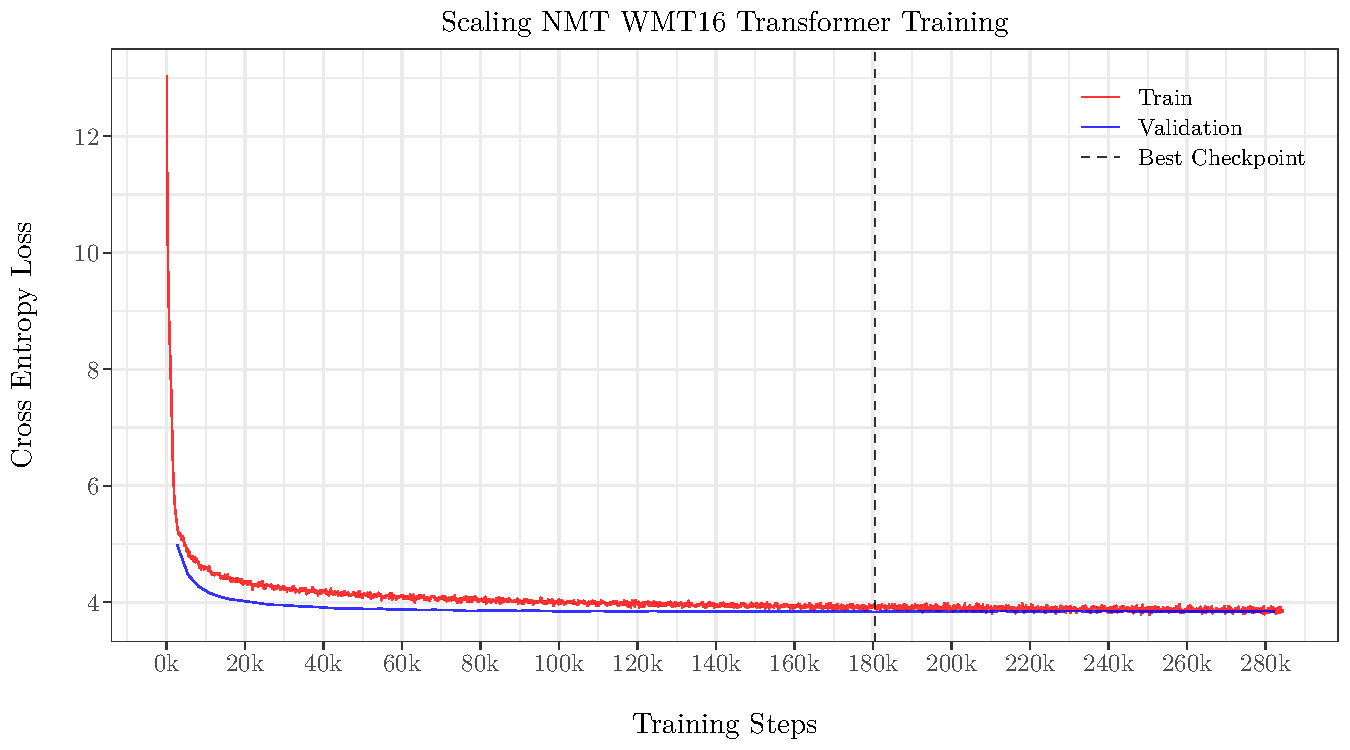
\includegraphics[trim={0cm 0cm 0cm 0cm},clip,width=\textwidth]{transformer_nmt_evolution.pdf}
  \caption{Training and validation cross entropy loss against training steps for Scaling NMT WMT16 Transformer}
  \label{transformer_nmt_evolution}
\end{figure*}

The PAWS data set contains 108,463 paraphrase and non-paraphrase sentence pairs with high lexical overlap. These sentence pairs were bulk sourced from Wikipedia and Quora Question Pairs; followed by controlled word swapping and back translation to create challenging sentence pairs for paraphrase detection. The generated sentence pairs were finally evaluated for fluency and general quality by human raters \cite{zhang2019paws}.

As noted in \citet{pawsx2019emnlp}, one limitation of adversarially generated data sets such as PAWS is their pre-dominant focus on the English language. In order to address this issue, \citet{pawsx2019emnlp} released PAWS-X; which consists of 23,659 human translated evaluation sentence pairs and 296,406 machine-translated training sentence pairs whose source sentences were derived from the Wikipedia subset of the original PAWS data set. These sentence pairs were translated from English to six typologically distinct languages; namely French, Spanish, German, Chinese, Japanese and Korean.

The release of PAWS-X provides many advantages to the field of NLP, particularly the creation of a new benchmark to promote research in multilingual and zero-shot paraphrase detection. This can already be seen by the incorporation of PAWS-X into Google's recent Cross-lingual TRansfer Evaluation of Multilingual Encoders (XTREME) benchmark system \cite{hu2020xtreme}.

\subsubsection{WMT16 de$\rightarrow$en}

In our research, we replicate a non-SOTA NMT model from scratch based off the Scaling NMT WMT16 workflow \cite{ott2018scaling}. While the original implementation in \citet{ott2018scaling} is based on the \texttt{en$\rightarrow$de} translation direction, our implementation trains a NMT model in the reverse translation direction; specifically \texttt{de$\rightarrow$en}.

For this, we use WMT16 \texttt{de$\rightarrow$en} training data with 4.5M sentence pairs, \texttt{newstest2013} as our validation set and \texttt{newstest2014} as our test set. We utilize a vocabulary of 32K symbols based off a joint source and target byte-pair encoding (BPE; \citealt{sennrich2015neural}).   

\subsection{Models}

\subsubsection{FAIR WMT19 Transformer}

We utilize FAIR's winning WMT19 single Transformer model as our SOTA NMT model. Focusing particularly on the \texttt{de$\rightarrow$en} translation direction, the FAIR WMT19 Transformer was the top performing model in WMT19 with a SacreBLEU \cite{post-2018-call} score of 40.8.

As per \citet{ng2019facebook}, the key factors that led to SOTA performance include \texttt{langid} filtering of crawled bitext data, large-scale back translation as a form of data augmentation and noisy channel model reranking. We utilized this model directly from \texttt{fairseq} \cite{ott2019fairseq}. 

\subsubsection{Scaling NMT WMT16 Transformer}

We replicate the Scaling NMT WMT16 Transformer based on \citet{ott2018scaling} by training it from scratch. However, we reverse the original translation direction from \texttt{en$\rightarrow$de} to \texttt{de$\rightarrow$en}; such that we can ultimately use this model to translate WMT19 paraphrases from \texttt{de$\rightarrow$en}. We intentionally choose this workflow since it would produce a non-SOTA transformer which would be useful for us downstream to introduce performance-dependent variance in the translation of WMT19 paraphrases.

\begin{figure*}
  \centering 
  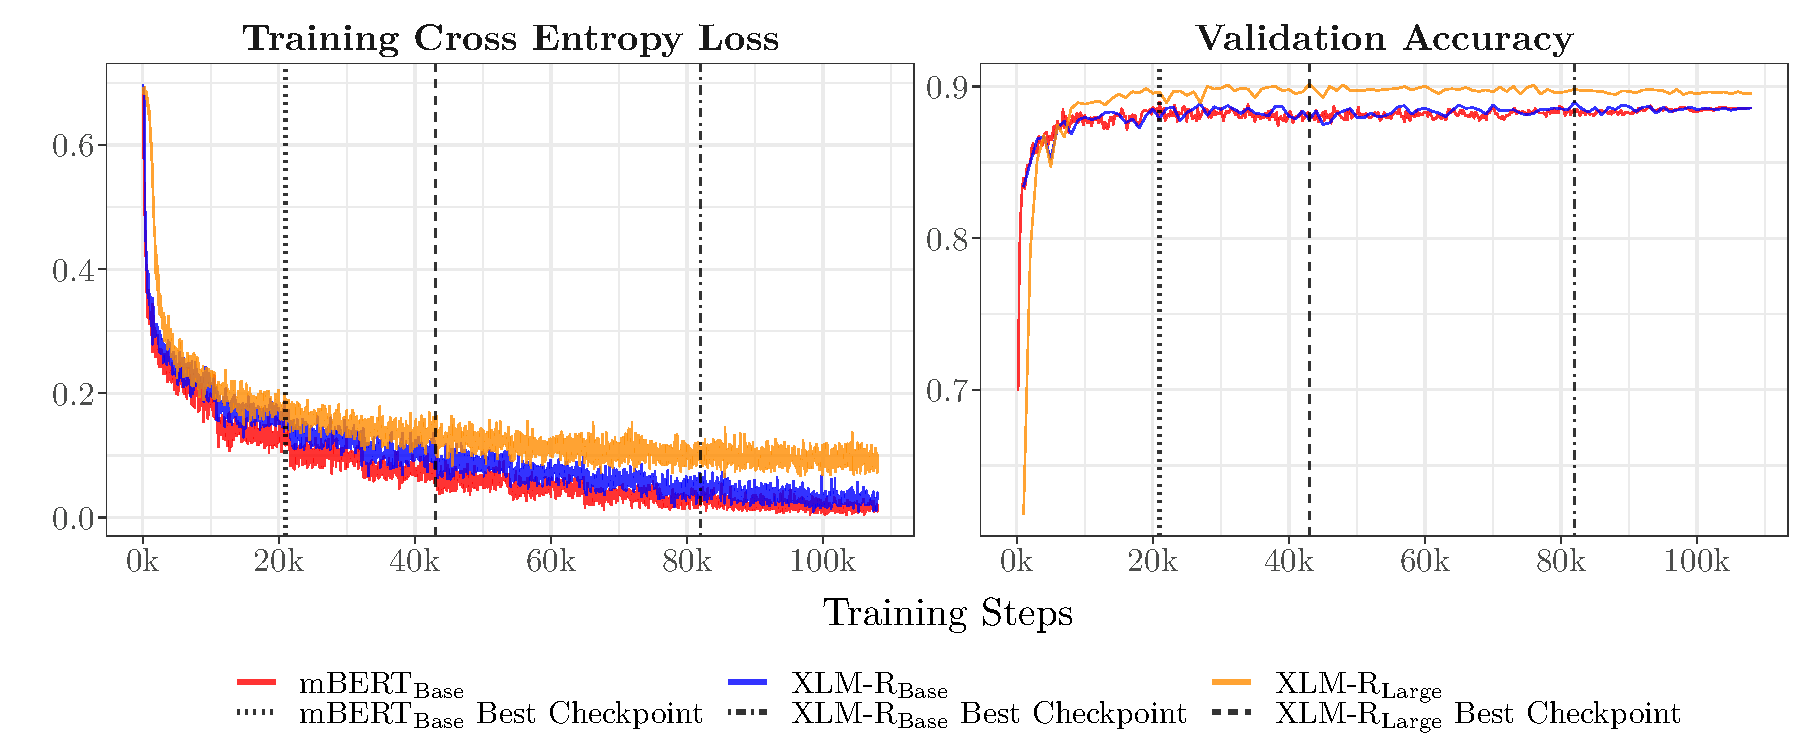
\includegraphics[trim={0.7cm 0cm 0cm 0cm},clip,width=\textwidth]{paraphrase_detection_models_evolution.pdf}
  \caption{Training cross-entropy loss and validation accuracy against training steps for paraphrase detection models}
  \label{paraphrase_detection_model_evolution}
\end{figure*}

Besides the aforementioned modification, we follow the same setup as per \citet{ott2018scaling}. Specifically, we use a ``big'' transformer model based off \citet{vaswani2017attention}; with 6 blocks in the encoder and decoder networks. This model has a total of 210M parameters.

During training, we apply dropout \cite{srivastava2014dropout} with probability 0.3 and utilize the Adam optimizer \cite{kingma2014adam} with $\beta_1 = 0.9$ and $\beta_2=0.98$. We use a learning rate schedule where the learning rate increases linearly for 4,000 steps from 1e-7 until 1e-3. The learning rate then decays proportionally to the inverse square root of the number of training steps. We utilize label smoothing with weight 0.1 for the uniform prior distribution over the vocabulary \cite{pereyra2017regularizing}. We use large batch sizes with the maximum number of tokens per batch being 7168. Furthermore, we apply gradient accumulation for 8 steps before updating the model. We also exploit \texttt{fairseq}'s half precision floating point (FP16) functionality for more efficient training.

Finally, we train this model for 6 days on a single NVIDIA Tesla V100 16GB GPU. During training, we monitor the validation loss and enable checkpoint-saving for the best performing checkpoint on the validation set. We train the model up until $\sim$285K updates.

Our best performing checkpoint is saved at $\sim$180K updates as seen in Figure \ref{transformer_nmt_evolution}. For evaluation on the test set, we utilize beam search with a beam width of 5. Our final Scaling NMT WMT16 Transformer achieved a SacreBLEU \cite{post-2018-call} score\footnote{\footnotesize SacreBLEU signature:\\BLEU+case.mixed+lang.de\nobreakdash-en+numrefs.1+smooth.exp+\\test.wmt14/full+tok.13a+version.1.4.12} of 31.0 on the \texttt{newstest2014} test set.

\subsubsection{Paraphrase detection models}

As noted in equation \ref{bounded_isometry_probability_eqn}, paraphrase detection models are useful in computing probabilistic binary semantic equivalence spaces, or otherwise the $S_L$ function. We follow a similar framework as per Google's XTREME benchmark \cite{hu2020xtreme} and fine-tune pre-trained multilingual transformer language models on the PAWS-X paraphrase detection task. We focus specifically on three multilingual transformer language models, specifically mBERT\textsubscript{Base} (104 languages; 172M parameters; \citealt{devlin-etal-2019-bert}), XLM-R\textsubscript{Base} (100 languages; 270M parameters; \citealt{conneau2019unsupervised}) and XLM-R\textsubscript{Large} (100 languages; 550M parameters; \citealt{conneau2019unsupervised}) using HuggingFace's \texttt{transformers} library \cite{Wolf2019HuggingFacesTS} with model variants optimized for sequence classification.

While our implementation is similar to that of Google's XTREME benchmark, we modify some aspects of the workflow to suit our needs. Most importantly, we fine-tune our multilingual language models on PAWS-X training data from all 7 languages instead of only English in order to reap the benefits of diverse multilingual data.

\begin{table}
  \centering
  \begin{tabular}{llll}
    \hline
    \textbf{Language} & \textbf{mBERT\textsubscript{B}} & \textbf{XLM-R\textsubscript{B}} & \textbf{XLM-R\textsubscript{L}} \\
    \hline
    en & 0.940 & 0.946 & 0.960 \\
    de & 0.898 & 0.900 & 0.912 \\
    es & 0.908 & 0.922 & 0.928 \\
    fr & 0.922 & 0.917 & 0.933 \\
    ja & 0.836 & 0.836 & 0.859 \\
    ko & 0.841 & 0.847 & 0.870 \\
    zh & 0.854 & 0.861 & 0.876 \\
    \hline \hline
    $\mu$ & 0.886 & 0.890 & \textbf{0.906} \\
    \hline
  \end{tabular} 
  \caption{Language-specific summary of macro-F\textsubscript{1} scores of paraphrase detection models on the PAWS-X test set; languages are abbreviated based on ISO 639-1; B and L refer to base and large respectively}
  \label{pawsx_score_breakdown}
\end{table}

For all models, we enforce a maximum sequence length of 128 tokens since PAWS-X sentence pairs generally fit it into this range. We use a modified Adam optimizer with decoupled weight decay regularization \cite{DBLP:journals/corr/abs-1711-05101} with $\beta_1 = 0.9$ and $\beta_2=0.999$. We train all models for 10 epochs or $\sim$110K updates with a global batch size of 32. We also use a linearly decaying learning rate schedule without warmup steps. Lastly, we monitor accuracy on the PAWS-X validation set for all languages in order to determine the best performing checkpoint.

Specific to mBERT\textsubscript{Base} and XLM-R\textsubscript{Base}, we use a batch size of 32 without gradient accumulation and an initial learning rate of 2e-5. As for XLM-R\textsubscript{Large}, we use an initial learning rate of 1e-6 and local batch size of 8 with 4 gradient accumulation steps to curb GPU out-of-memory (OOM) issues.

We fine-tune mBERT\textsubscript{Base}, XLM-R\textsubscript{Base} and XLM-R\textsubscript{Large} for 14 hours, 15 hours and 2.5 days on a single NVIDIA GeForce GTX 1080 Ti 12GB GPU respectively. The best performing checkpoints are saved at $\sim$20K, $\sim$80K and $\sim$40K updates respectively, as seen in Figure \ref{paraphrase_detection_model_evolution}.

As seen in Table \ref{pawsx_score_breakdown}, all three models perform well; especially on English and German. Overall, the best performing model on the PAWS-X test set is XLM-R\textsubscript{Large} with a macro-F\textsubscript{1} of 0.906.

\subsection{Evaluation protocols}

Given our German WMT19 Legacy and WMT19 AR paraphrase data sets defined in equations \ref{wmt19legacy} and \ref{wmt19ar}, we translate all pairs of paraphrases using both the FAIR WMT19 and the Scaling NMT WMT16 Transformers in the \texttt{de$\rightarrow$en} translation direction with a beam width of 5. With this, we utilize the source German paraphrases along with their target-side English translations for further investigation. 

\subsubsection{Isometry on binary semantic equivalence spaces}

\paragraph{Vector representation:} We modify our representation of the $S_L$ relations in equation \ref{exact_approx_isometry_eqn} in order to have a more concise vectorized form of the relationship. We assign the probability threshold $\epsilon$ from equation \ref{bounded_isometry_probability_eqn} a constant value of 0.5 for all computations of $S_L$ in this research:

\vspace{-5pt}
\begin{gather}
  \mathbf{S_{XY}} = \begin{bmatrix} S_X(s_1, s_2) \\[5pt] S_Y(f(s_1), f(s_2)) \end{bmatrix} \\[10pt] 
  \mathbf{S_{XY}^{\mathsf{T}}} = \begin{bmatrix} S_X(s_1, s_2) & S_Y(f(s_1), f(s_2)) \end{bmatrix}
\end{gather}

\paragraph{Multi-model decisions:} Given this formulation of $\mathbf{S_{XY}^{\mathsf{T}}}$, it is worth noting that each of the three paraphrase detection models would compute a separate $\mathbf{S_{XY}^{\mathsf{T}}}$ term. Since our paraphrase detection models were evaluated to have non-zero (albeit small and similar) error rates, we decide to use the $\mathbf{S_{XY}^{\mathsf{T}}}$ outputs of all three models and compute the statistical mode of the three outputs. Such a majority decision would provide more confidence in any particular decision from the models. For simplicity, we assign the statistical mode function with the symbol $\mathbf{M}$. We therefore compute $\mathbf{M(S_{XY}^{\mathsf{T}}})$ to check for a majority decision over the three paraphrase detection models. We assign the empty set $\emptyset$ in case no majority decision exists.

\paragraph{Discrete possibilities:} Since the output of $S_L$ falls in the binary set of $\{0,1\}$, we can effectively compute all five possibilities of the consequent majority decision $\mathbf{M(S_{XY}^{\mathsf{T}}})$. We describe these in the context of binary semantic equivalence spaces.

\begin{figure*}
  \centering 
  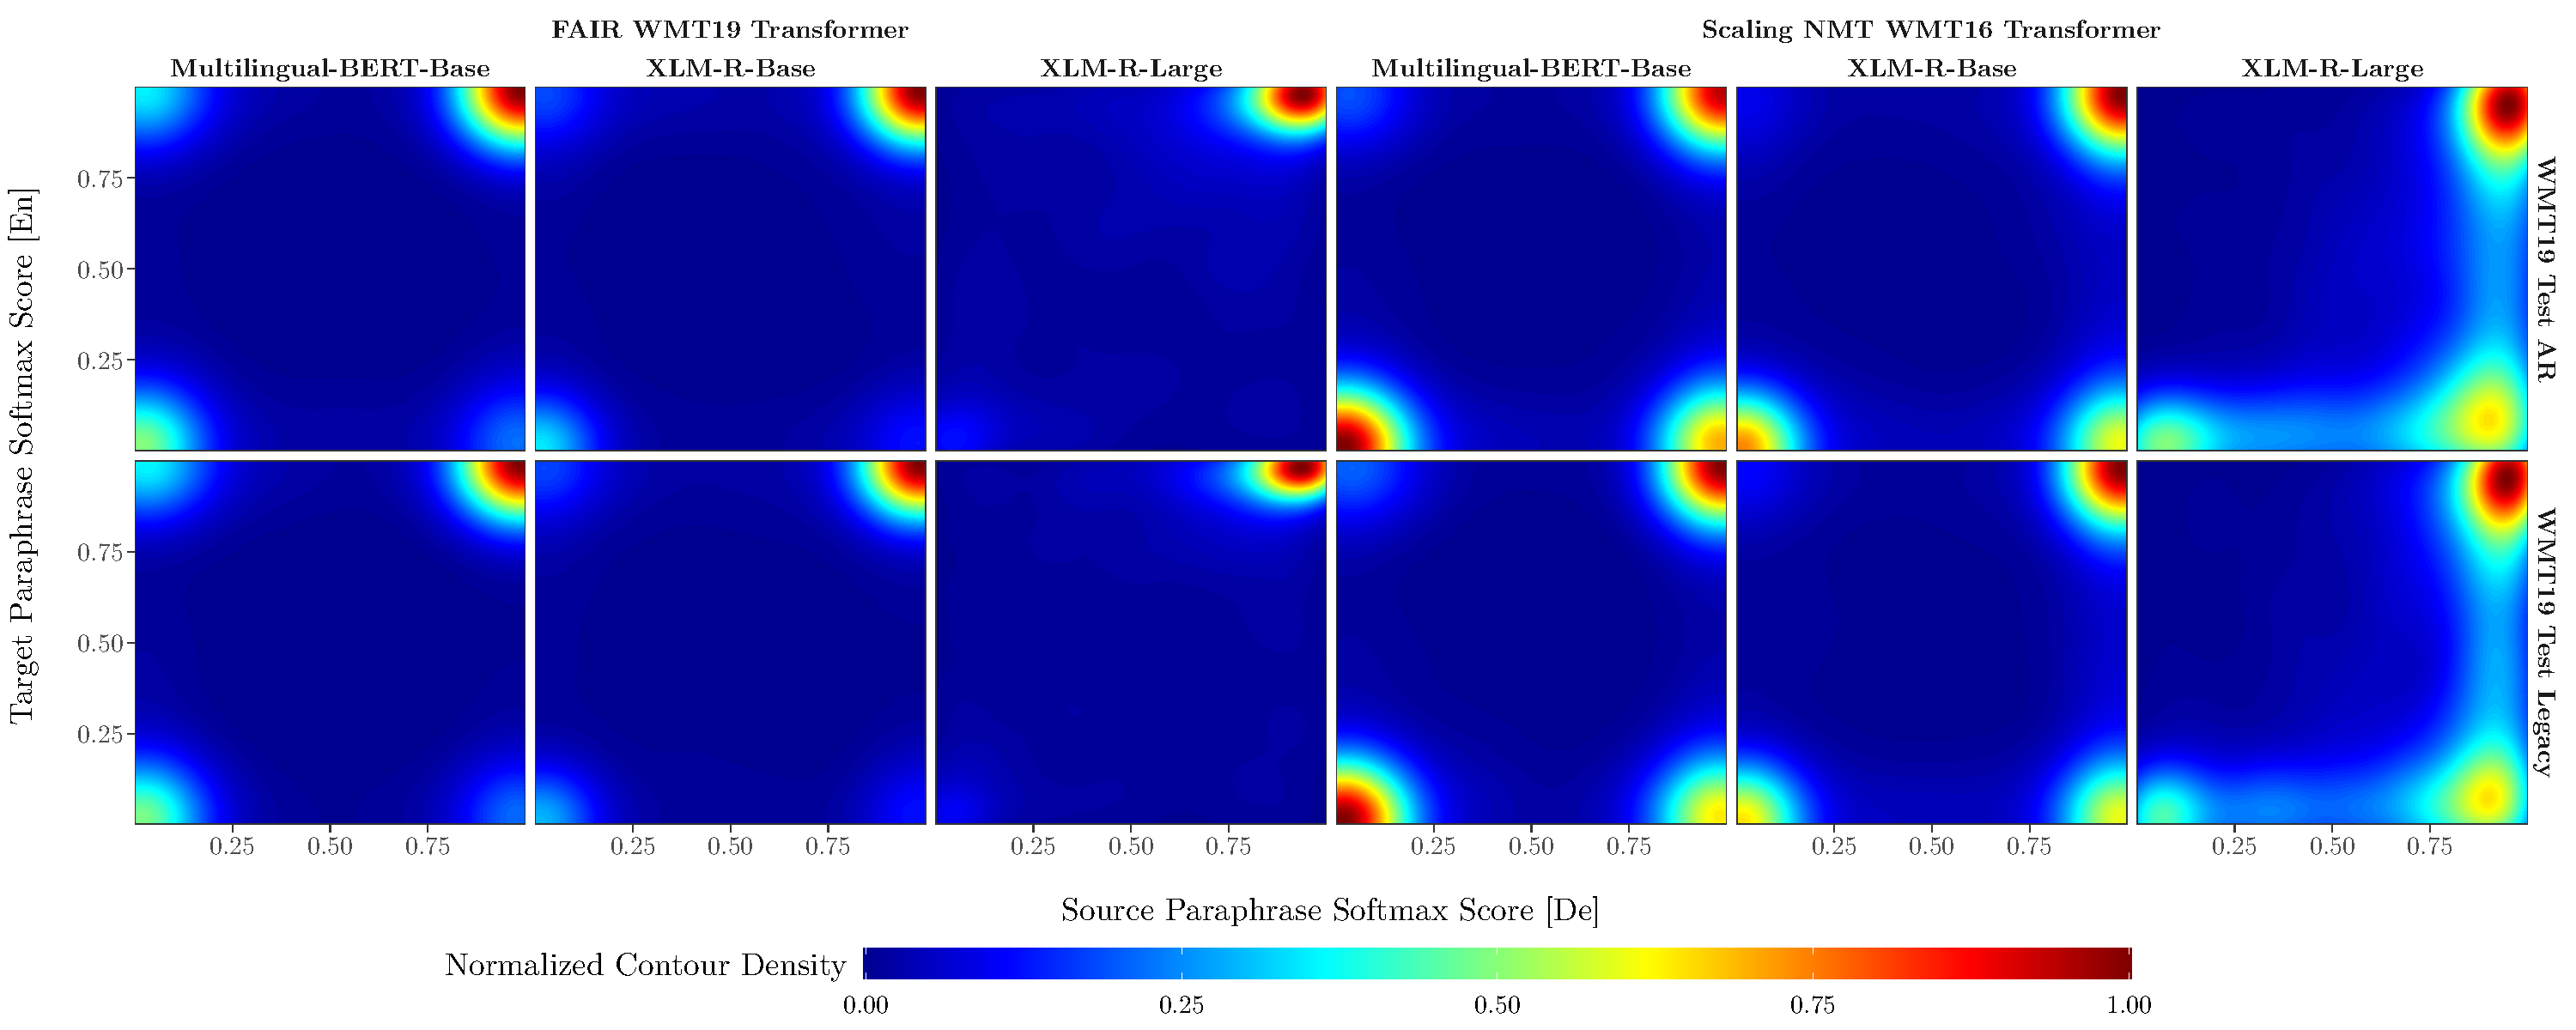
\includegraphics[trim={0cm 0cm 0cm 0cm},clip,width=\textwidth]{paraphrase_detection_softmax_all.pdf}
  \caption{Normalized contour densities for target paraphrase softmax score against source paraphrase softmax score by NMT models, paraphrase detection models and input data sets}
  \label{paraphrase_detection_softmax_all}
\end{figure*}

\begin{enumerate}
\item $\mathbf{M(S_{XY}^{\mathsf{T}}}) = [1, 1]$: Both the source and target pairs of sentences were evaluated to be paraphrases and are therefore semantically equivalent on both sides. This qualifies as \textit{isometric behaviour}.
\item $\mathbf{M(S_{XY}^{\mathsf{T}}}) = [0, 0]$: Both the source and target pairs of sentences were evaluated to be non-paraphrases and are therefore not semantically equivalent on both sides. While this does qualify as approximate isometry according to equation \ref{exact_approx_isometry_eqn}, we also observe this scenario is less conclusive for determining isometry compared to $\mathbf{M(S_{XY}^{\mathsf{T}}}) = [1, 1]$ because of a looser bound associated with $S_L=0$ as per equation \ref{bounded_isometry_eqn}. We therefore consider this behaviour to be \textit{ambiguous}.  
\item $\mathbf{M(S_{XY}^{\mathsf{T}}}) = [0, 1]$: The source sentences are evaluated to be non-paraphrases while the target sentences are evaluated to be paraphrases. This implies that translation resulted in the sentence pair becoming semantically equivalent while they were not before. This qualifies as anisometric behaviour and could be an interesting scenario to investigate further. We define this as \textit{type-1 anisometric behaviour}.
\item $\mathbf{M(S_{XY}^{\mathsf{T}}}) = [1, 0]$: The source sentences are evaluated to be paraphrases while the target sentences are evaluated to be non-paraphrases. This implies that translation resulted in the sentence pair becoming semantically inequivalent while they were not before. This qualifies as anisometric behaviour and could imply weak performance of the model on one of the sentences; or possibly some adversarial paraphrasing. We define this as \textit{type-2 anisometric behaviour}.
\item $\mathbf{M(S_{XY}^{\mathsf{T}}}) = \emptyset$: This implies that all models had different decisions and therefore no majority decision was reached. We consider this behaviour to be \textit{ambiguous}.
\end{enumerate}

\paragraph{Frequency analysis:} Given the five aforementioned possibilities of $\mathbf{M(S_{XY}^{\mathsf{T}}})$, we measure the frequency of each possibility for each model. This give us an insight into the semantically isometric behaviour of the models and would allow us to conduct comparisons across them.

\paragraph{Sentence-level analysis:} In order to check the veracity of the $\mathbf{M(S_{XY}^{\mathsf{T}}})$ outputs, we analyze selected individual sentence pairs and their target translations, and attempt to interpret these results.

\subsubsection{Relationship between chrF$_2$ and semantic equivalence}

We return to one of the observations from \citet{michel2019evaluation}, specifically that the chrF$_2$ automatic sequence evaluation metric \cite{popovic2015chrf} tends to correlate most positively with human judgment of semantic similarity compared to BLEU \cite{papineni2002bleu} and METEOR \cite{denkowski2014meteor}. We use our current research to further investigate the relationship between semantic equivalence and the chrF$_2$ automatic sequence evaluation metric. We replicate the chrF$_2$ setup from \citet{michel2019evaluation} by using the default \texttt{sacrebleu} implementation \cite{post-2018-call} with a $n$-gram upper limit of 6 and $\beta$ value of 2

\paragraph{Non-commutativity of chrF$_2$:} While replicating the chrF$_2$ setup of \citet{michel2019evaluation}, we observe that this particular formulation with $\beta = 2$ results in the chrF$_2$ metric being non-commutative, where $s_1$ and $s_2$ are input sentences:

\begin{equation}
  \text{chrF}_{2}(s_1,s_2) \neq \text{chrF}_{2}(s_2,s_1)
\end{equation}

\begin{figure*}
  \centering 
  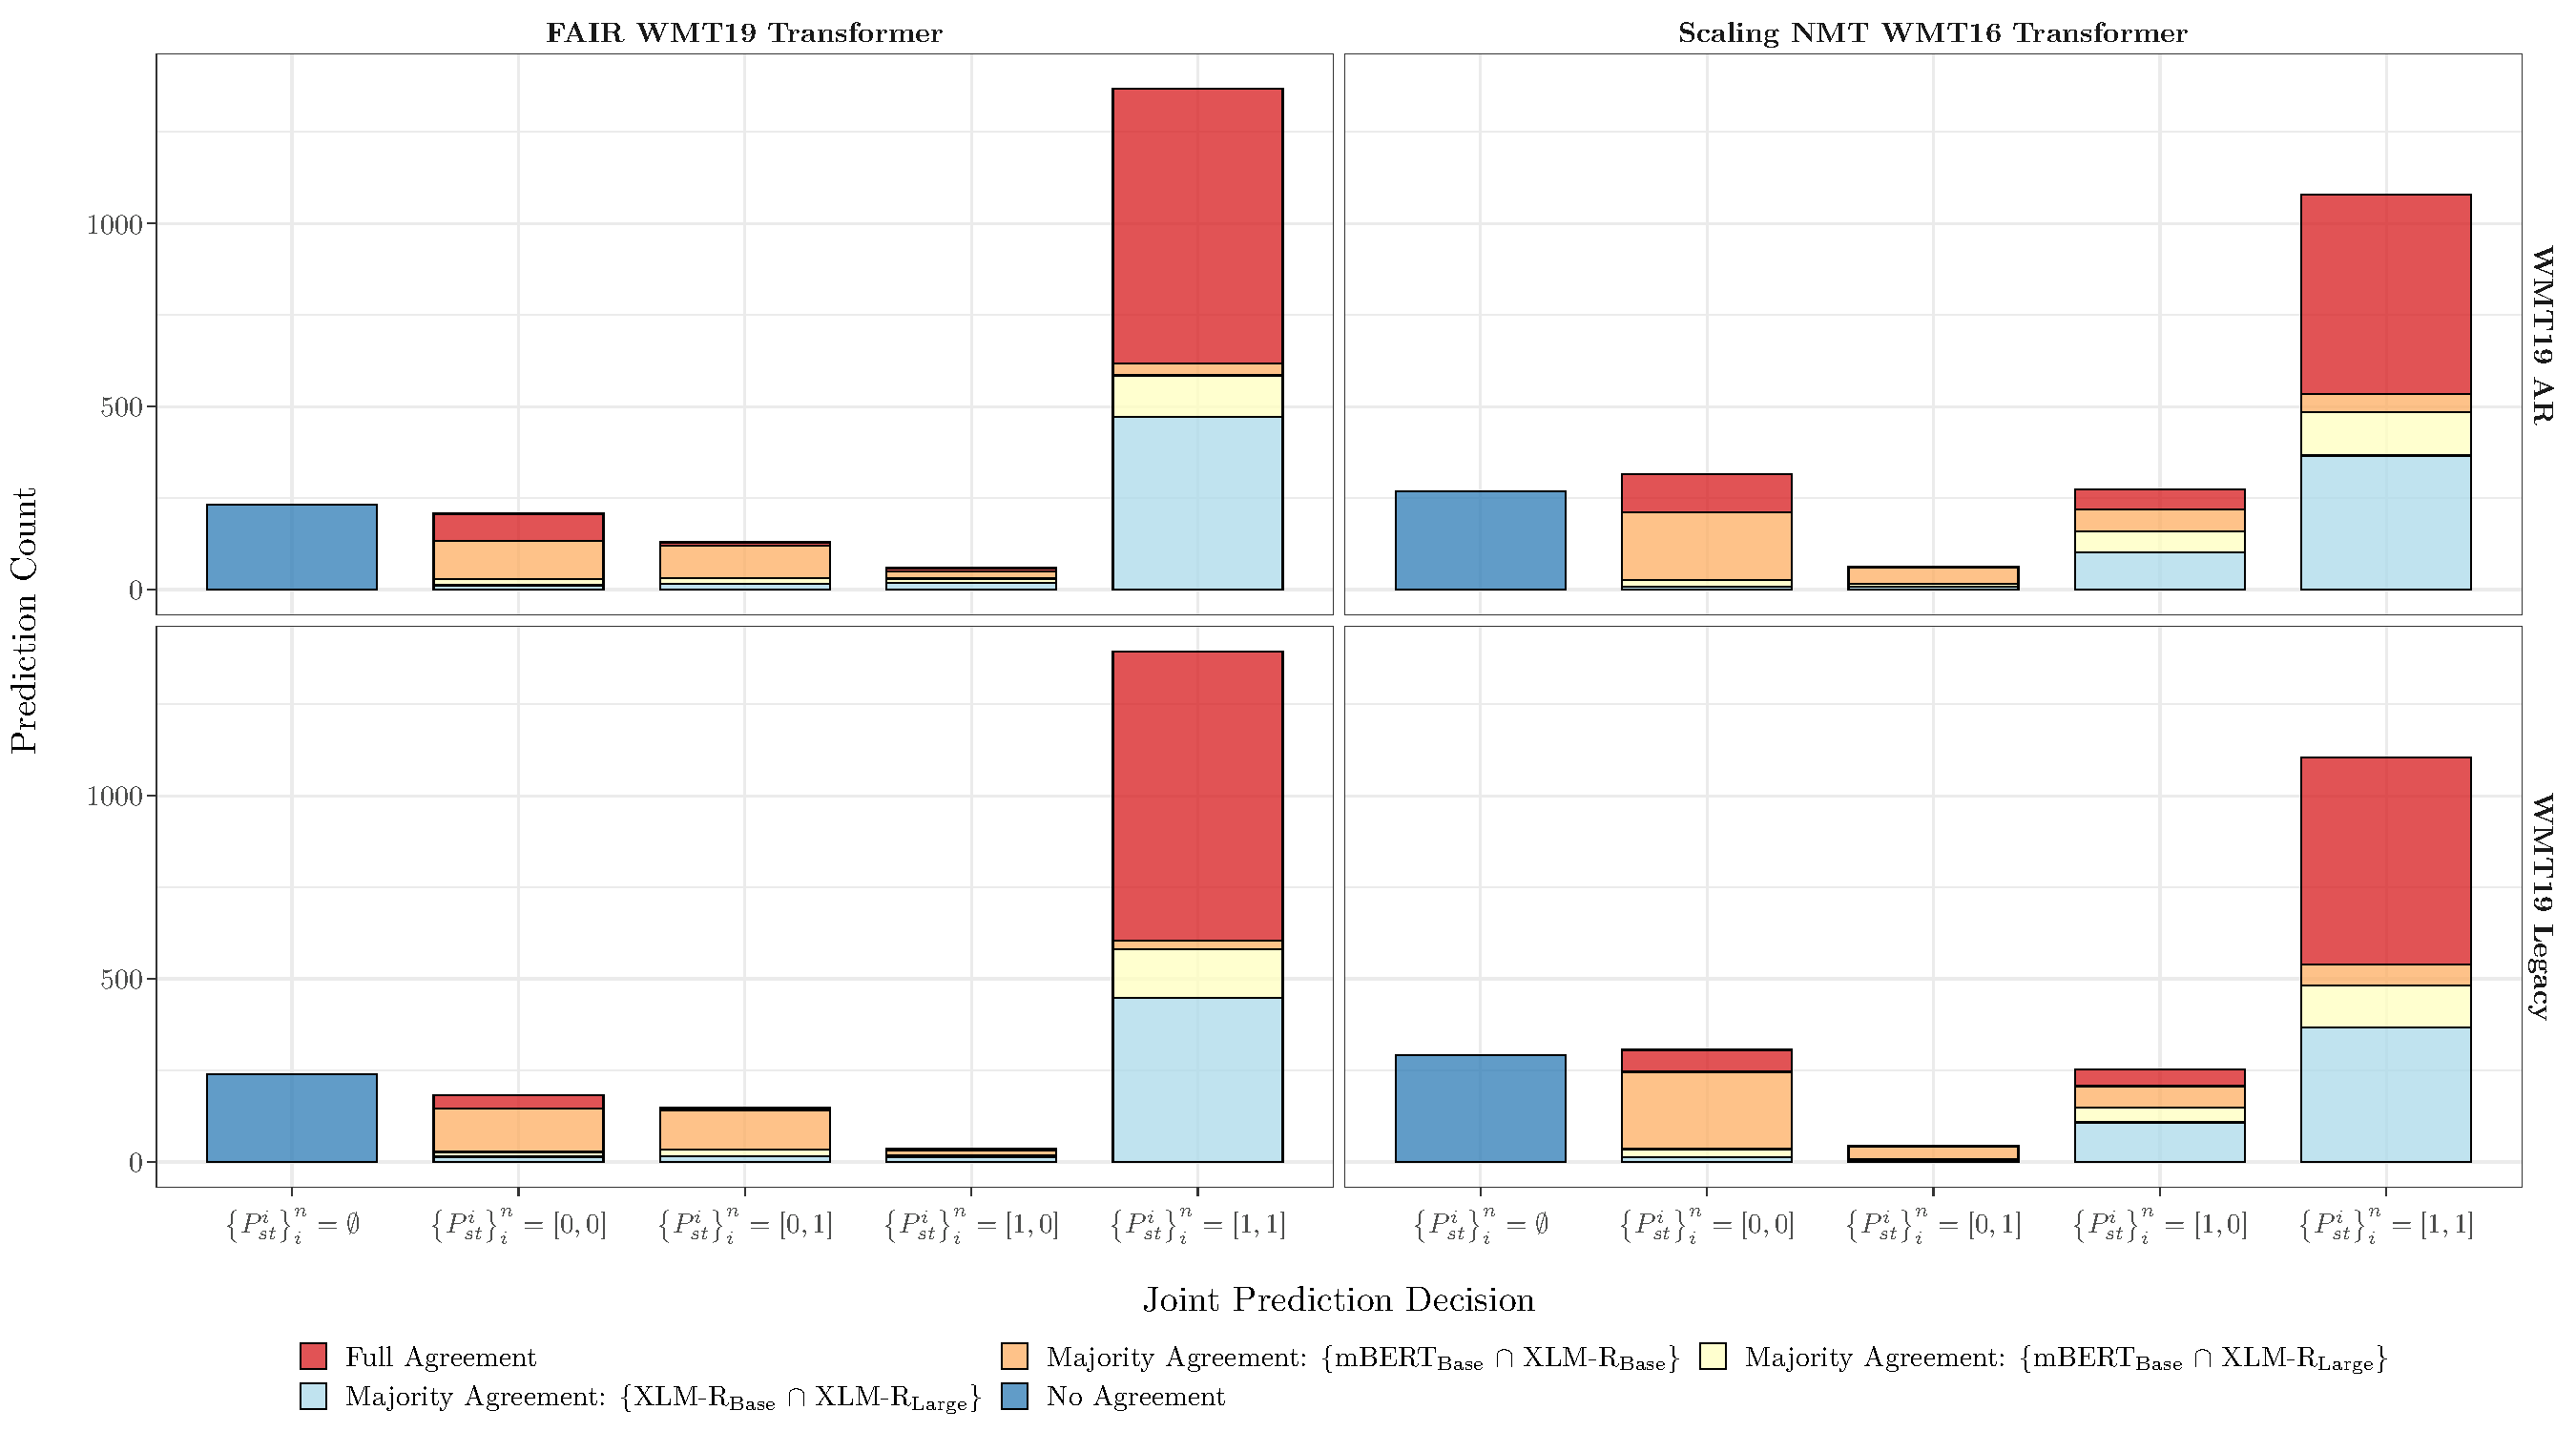
\includegraphics[trim={0cm 0cm 0cm 0cm},clip,width=\textwidth]{paraphrase_detection_joint_decision.pdf}
  \caption{Frequency distribution of $\mathbf{M(S_{XY}^{\mathsf{T}}})$ by NMT models and input data sets; filling colors indicate finer details on the type of majority decision}
  \label{paraphrase_detection_joint_decision}
\end{figure*}

\begin{table*}[t!]
  \centering
  \begin{tabular*}{\textwidth}{c @{\extracolsep{\fill}} cccccc}
    \hline \\[-10pt]
    \multirow{2}[3]{*}{$\mathbf{M(S_{XY}^{\mathsf{T}}})$} & \multicolumn{3}{c}{\textbf{FAIR WMT19 Transformer}} & \multicolumn{3}{c}{\textbf{Scaling NMT WMT16 Transformer}} \\
    \cmidrule(lr){2-4} \cmidrule(lr){5-7}
    & WMT19 Legacy & WMT19 AR & $\mu$ & WMT19 Legacy & WMT19 AR & $\mu$ \\[3pt]
    \hline \hline \\[-10pt]
    $[1,1]$ & \textbf{0.698} & \textbf{0.686} & \textbf{0.692} & 0.554 & 0.541 & 0.548 \\
    $[0,0]$ & 0.091 & 0.104 & 0.097 & 0.153 & 0.154 & 0.153 \\
    $[0,1]$ & \textbf{0.074} & \textbf{0.065} & \textbf{0.069} & 0.033 & 0.031 & 0.032 \\
    $[1,0]$ & 0.018 & 0.030 & 0.024 & \textbf{0.133} & \textbf{0.130} & \textbf{0.131}\\
    $\emptyset$ & 0.120 & 0.117 & 0.118 & 0.128 & 0.144 & 0.136 \\
    \hline
  \end{tabular*}
  \caption{Relative frequency distribution for $\mathbf{M(S_{XY}^{\mathsf{T}}})$ by NMT models and input data sets; $\mu$ indicates the macro-average of the relative frequency over the input data sets for each model}
  \label{isometry_frequency}
\end{table*}

Non-commutativity is an emergent property of chrF$_2$ with $\beta = 2$ since this would assign two times more weight to recall than precision \cite{popovic2015chrf}; which places an internal bias on input order. While this non-commutative formulation of chrF$_2$ would be useful for evaluating NMT models with explicit hypotheses and references, this would not be optimal as a semantic similarity metric since one would expect a semantic similarity metric to be commutative and unbiased towards input order.

\paragraph{Commutative variant of chrF$_2$:} As an alternative, we simulate commutativity by averaging the chrF$_2$ values for both input orders and introduce $\overline{\text{chrF}_2}$ as a commutative variant for chrF$_2$:

\begin{gather}
  \overline{\text{chrF}_2}(s_1,s_2) = \dfrac{\text{chrF}_2(s_1,s_2) + \text{chrF}_2(s_2,s_1)}{2} \\[5pt]
  \therefore \quad \overline{\text{chrF}_2}(s_1,s_2) = \overline{\text{chrF}_2}(s_2,s_1)
\end{gather}

We see this as a more optimal alternative than changing $\beta$ to 1 since this might veer further away from the experimental setup of \citet{michel2019evaluation}. Such commutative variants of automatic sequence evaluation metrics have also been considered for BLEU and METEOR in \citet{wieting-etal-2019-beyond} and were termed symmetric instead of commutative.

\paragraph{Mapping $\overline{\text{chrF}_2}$ to $S_L$:}
We refer back to the majority decisions of the paraphrase detection models and remove all sentence pairs where $\mathbf{M(S_{XY}^{\mathsf{T}}}) = \emptyset$. We assume all remaining sentence pairs have been confidently tagged by the paraphrase detection models. We assign the remaining sentence pairs with their respective $\overline{\text{chrF}_2}$ and $S_L$ values for the source and target sides. 

\paragraph{Correlation between $\overline{\text{chrF}_2}$ and $S_L$:} Finally, we replicate a similar statistical procedure as per \citet{michel2019evaluation} and compute the Pearson correlation coefficient $r_{xy}$ and a corresponding statistical $t$-test. For the $t$-test, we set the null hypothesis $H_0$ to be that there exists a non-positive correlation between $\overline{\text{chrF}_2}$ and $S_L$; while the alternative hypothesis $H_1$ is that there exists a positive correlation between $\overline{\text{chrF}_2}$ and $S_L$. We interpret the strength of correlations using guidelines from \citet{schober2018correlation}.     

\begin{figure*}
  \centering 
  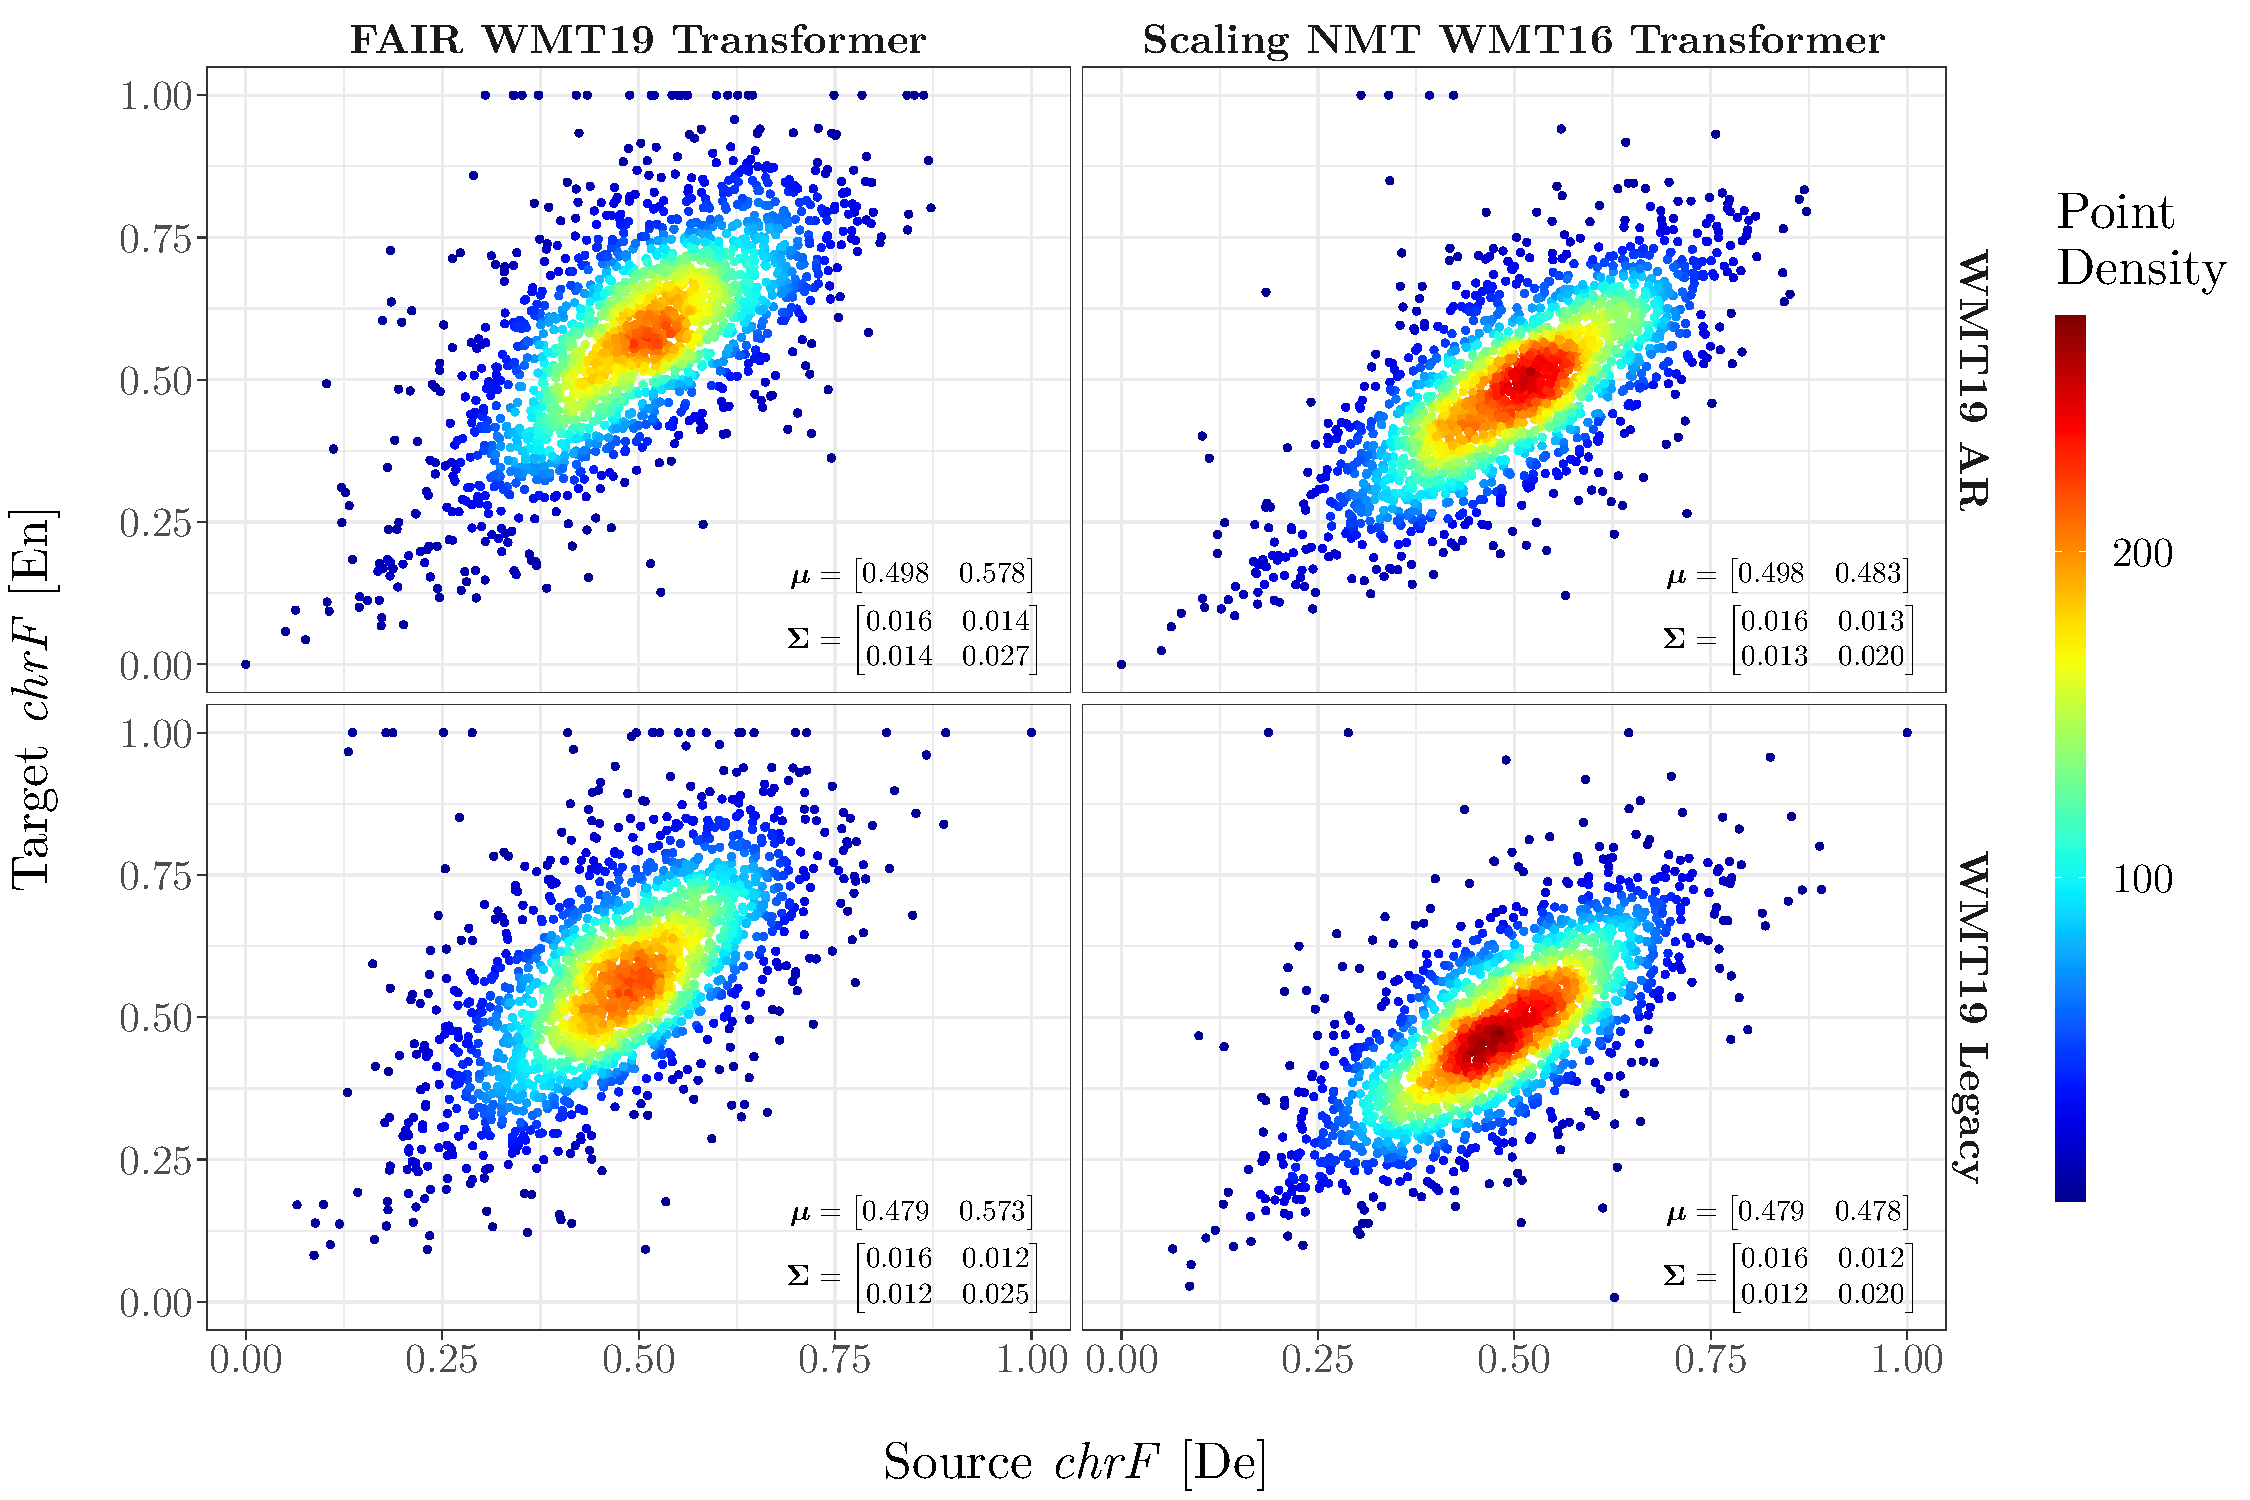
\includegraphics[trim={0cm 0cm 0cm 0cm},clip,width=\textwidth]{chrf_nmt.pdf}
  \caption{Distributions of target-side $\overline{\text{chrF}_2}$ against source-side $\overline{\text{chrF}_2}$ by NMT models and input data sets}
  \label{chrf_distribution}
\end{figure*}

\section{Results}

\subsection{Isometry on binary semantic equivalence spaces}

\subsubsection{Paraphrase detection softmax scores}

Figure \ref{paraphrase_detection_softmax_all} shows a normalized contour density estimate for paraphrase detection softmax scores. These scores are grouped by NMT models, input data sets and paraphrase detection models. We observe that mBERT\textsubscript{Base} generally shows more variance in softmax scores compared to the XLM-R models. We can also observe that all models show more variance for translation outputs from the Scaling NMT WMT16 Transformer compared to those from the FAIR WMT19 Transformer. The softmax distributions are generally similar between the WMT19 Legacy and WMT19 AR input data sets.

\subsubsection{Frequency analysis}

Figure \ref{paraphrase_detection_joint_decision} shows a visual breakdown of absolute frequencies of $\mathbf{M(S_{XY}^{\mathsf{T}}})$ by NMT models and input data sets. Table \ref{isometry_frequency} shows a tabular breakdown of relative frequencies of $\mathbf{M(S_{XY}^{\mathsf{T}}})$ by NMT models and input data sets. Below are the key observations in the context of binary semantic equivalence spaces.

\paragraph{Isometry:} We observe a higher proportion of isometric behaviour with the FAIR WMT19 Transformer (69.2$\%$) compared to the Scaling NMT WMT16 Transformer (54.8$\%$).
\paragraph{Type-1 anisometry:} We observe a higher proportion of type-1 anisometric behaviour with the FAIR WMT19 Transformer (6.9$\%$) compared to the Scaling NMT WMT16 Transformer (3.2$\%$).
\paragraph{Type-2 anisometry:} We observe a lower proportion of type-2 anisometric behaviour with the FAIR WMT19 Transformer (2.4$\%$) compared to the Scaling NMT WMT16 Transformer (13.1$\%$).  
\paragraph{Ambiguity:} We observe a lower proportion of ambiguous samples with the FAIR WMT19 Transformer (21.5$\%$) compared to the Scaling NMT WMT16 Transformer (28.9$\%$).
\paragraph{Model agreement:} Based on Figure \ref{paraphrase_detection_joint_decision}, we observe that the majority of agreements are full agreements, followed by XLM-R\textsubscript{Base} and XLM-R\textsubscript{Large} agreements, mBERT\textsubscript{Base} and XLM-R\textsubscript{Base} agreements and finally mBERT\textsubscript{Base} and XLM-R\textsubscript{Large} agreements.

\subsection{Correlation between $\overline{\text{chrF}_2}$ and $S_L$}

\subsubsection{Source and target $\overline{\text{chrF}_2}$ distributions}

Figure \ref{chrf_distribution} shows the distribution of $\overline{\text{chrF}_2}$ over the source and target sides, grouped over NMT models and input data sets. We observe a larger variance of $\overline{\text{chrF}_2}$ points for the FAIR WMT19 Transformer outputs compared to those from the Scaling NMT WMT16 Transformer.

Furthermore, we can observe a larger mean $\overline{\text{chrF}_2}$ value for the FAIR WMT19 Transformer compared to the Scaling NMT WMT16 Transformer. This can be inferred from the general distribution of points from the former being above the diagonal compared to those from the latter being centered near the diagonal. We can also observe more cases where $\overline{\text{chrF}_2} = 1$ on the target side but $\overline{\text{chrF}_2} \neq 1$ on the source side for the FAIR WMT19 Transformer compared to the Scaling NMT WMT16 Transformer. 

\begin{figure*}
  \centering 
  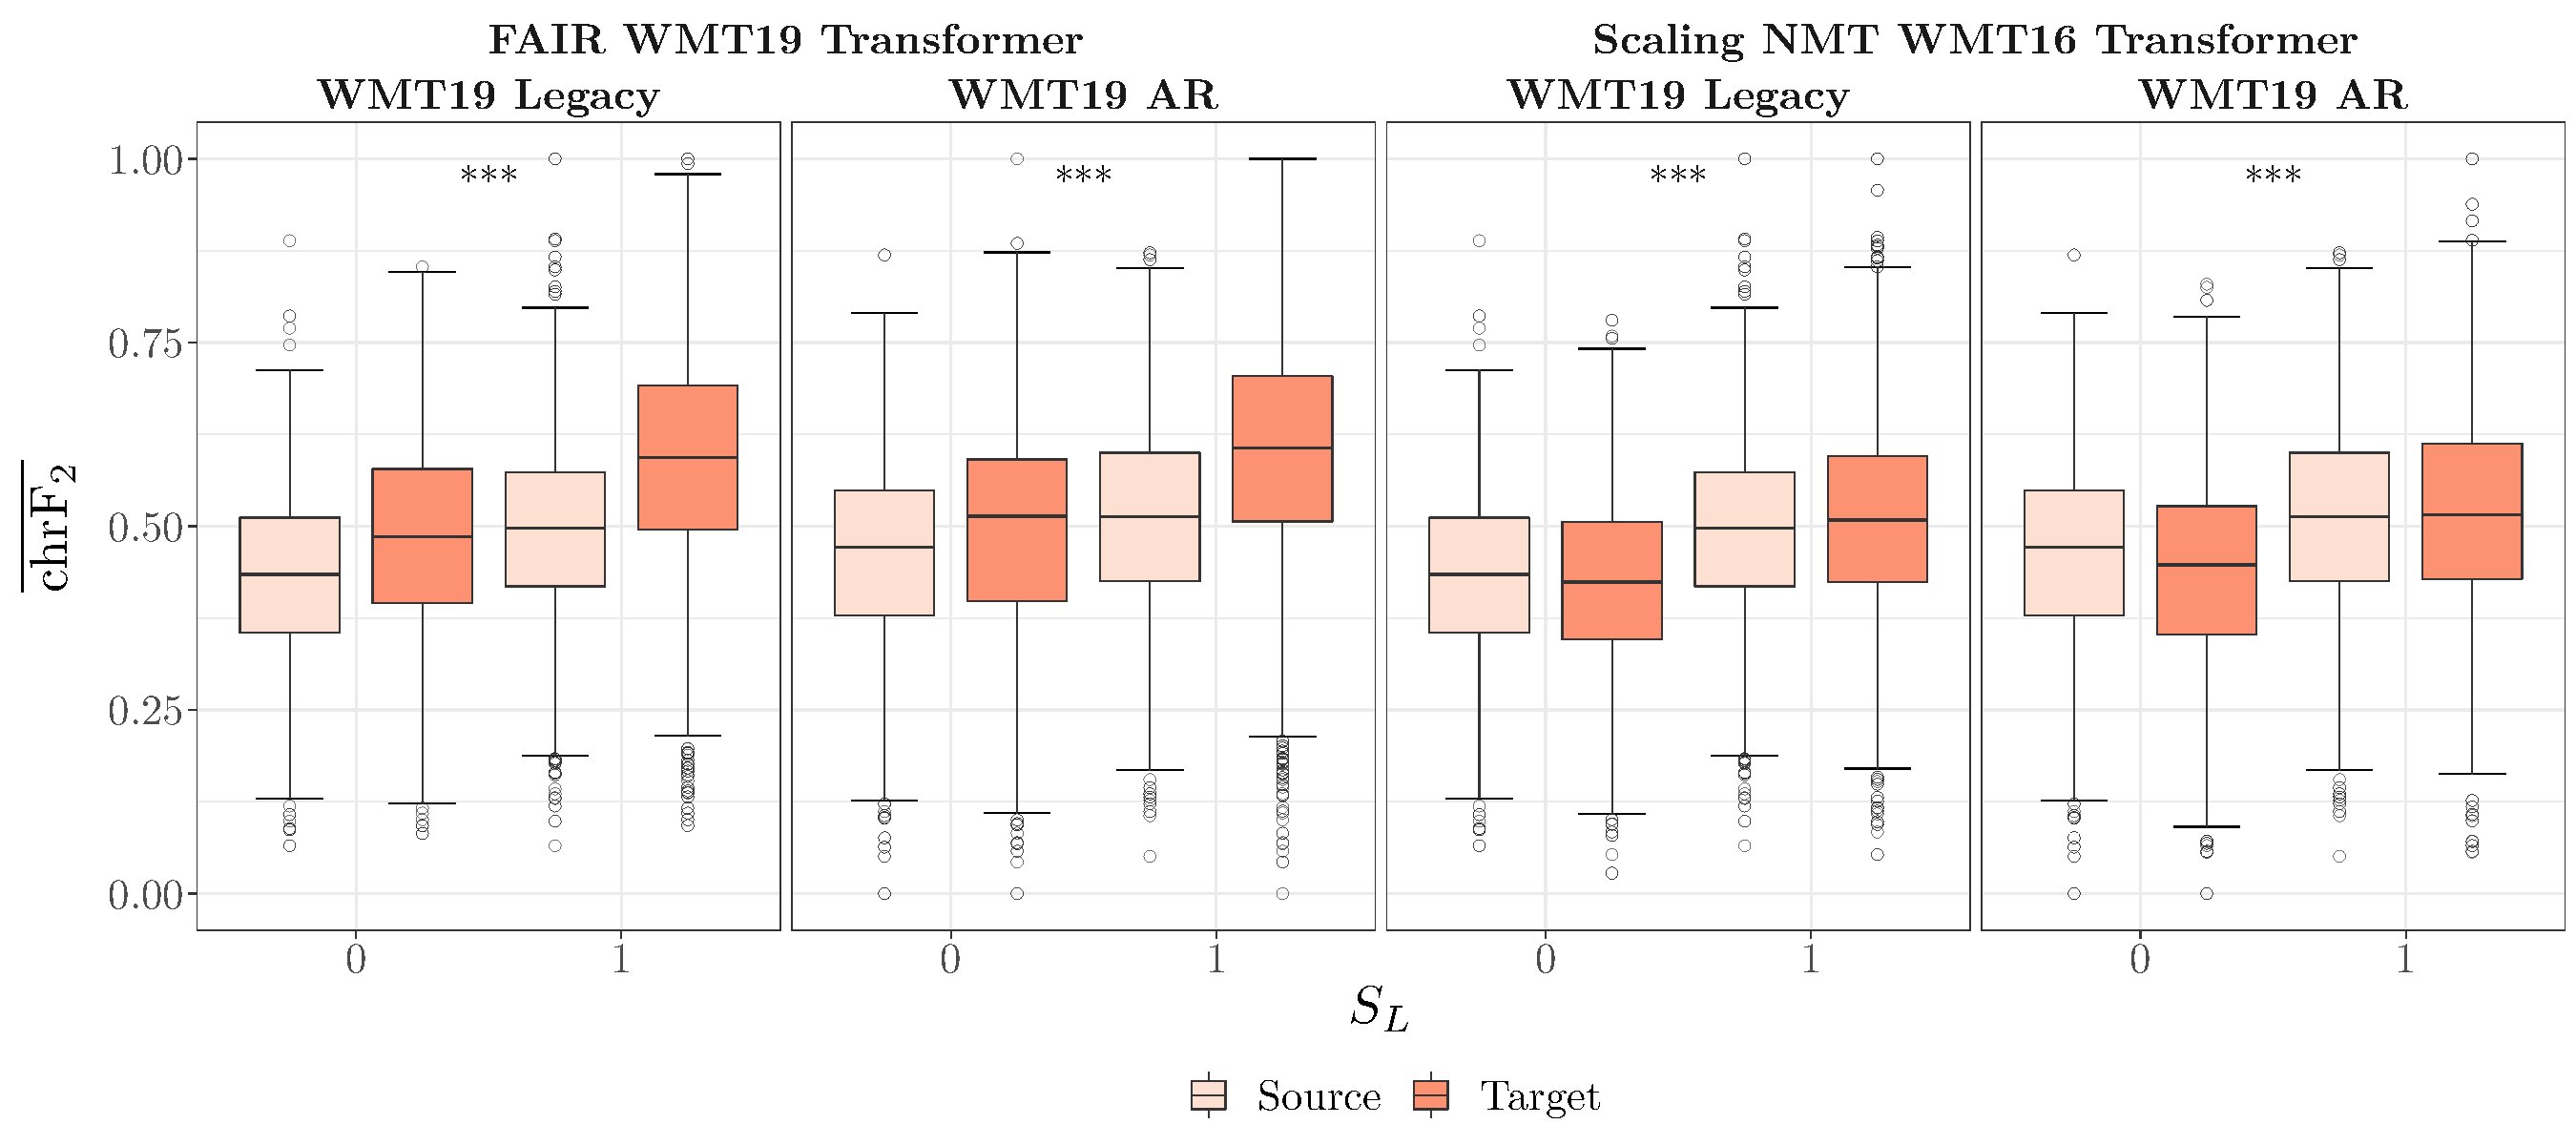
\includegraphics[trim={0.25cm 0cm 0cm 0cm},clip,width=\textwidth]{chrf_paraphrase_detection_boxplot_joint_decision.pdf}
  \caption{Distributions of $\overline{\text{chrF}_2}$ against $S_L$ by NMT models and input data sets ; *** indicates a statistically significant positive correlation between $\overline{\text{chrF}_2}$ and $S_L$ with $p \leq 0.001$ for the one-tailed $t$-test}
  \label{chrf_paraphrase_detection_joint_boxplot}
\end{figure*}

\begin{table*}[t!]
  \centering
  \begin{tabular*}{\textwidth}{c @{\extracolsep{\fill}} cccccc}
    \hline \\[-10pt]
    \multirow{2}[3]{*}{Statistic} & \multicolumn{3}{c}{\textbf{FAIR WMT19 Transformer}} & \multicolumn{3}{c}{\textbf{Scaling NMT WMT16 Transformer}} \\
    \cmidrule(lr){2-4} \cmidrule(lr){5-7}
    & WMT19 Legacy & WMT19 AR & $\mu$ & WMT19 Legacy & WMT19 AR & $\mu$ \\[3pt]
    \hline \hline \\[-10pt]
    $r_{xy}$ & 0.269 & 0.243 & \textbf{0.256} & 0.269 & 0.231 & \textbf{0.250} \\[3pt]
    $H_1: r>0$ & *** & *** & \textemdash & *** & *** & \textemdash \\[5pt]
    \hline \\[-10pt]
    Correlation & Weak & Weak & \textemdash & Weak & Weak & \textemdash \\[2pt]
    \hline
  \end{tabular*}
  \caption{Tabular summary of Pearson correlation coefficients $r_{xy}$, $t$-test alternative hypothesis and correlation strength interpretation \cite{schober2018correlation} by NMT models and input data sets; *** indicates $p\leq0.001$ for the one-tailed $t$-test}
  \label{chrf_correlation}
\end{table*}

\subsubsection{Correlation analysis}

Figure \ref{chrf_paraphrase_detection_joint_boxplot} shows the distribution of $\overline{\text{chrF}_2}$ against $S_L$ by over NMT models, input data sets and source-target origins. Table \ref{chrf_correlation} shows a breakdown of Pearson correlation coefficients $r_{xy}$ for $\overline{\text{chrF}_2}$ and $S_L$ and results of the statistical $t$-test by NMT models and input data sets.

Overall, we observe a significant positive correlation between $\overline{\text{chrF}_2}$ and $S_L$ with mean Pearson correlation coefficient $r_{xy}$ values of $0.256$ and $0.250$ for the FAIR WMT19 Transformer and the Scaling NMT WMT16 Transformer respectively. The one-tailed $t$-test used to ascertain significance showed a strongly significant positive correlation with $p\leq0.001$. According to the interpretation guidelines from \citet{schober2018correlation}, this range of $r_{xy}$ would imply a weak correlation strength between $\overline{\text{chrF}_2}$ and $S_L$. 

\section{Discussion}

\subsection{Isometry on binary semantic equivalence spaces}

\begin{table*}[t!]
  \centering
  \begin{tabular*}{\textwidth}{ll p{5.9cm} p{5.9cm}}
    \hline \\[-10pt]
    $\mathbf{M(S_{XY}^{\mathsf{T}}})$ & Type & Sentence in WMT19 AR & Paraphrase in WMT19 AR \\[5pt]
    \hline \hline \\[-10pt]
    $[1,1]$ & \textcolor{red}{Source} & Glocken von St. Martin verstummen, da Kirchen in Harlem kämpfen &  St. Martin‘s Glocken läuten nicht mehr, weil in Harlem ein Kampf der Kirchen in Gang ist \\\\[-5pt]
                                      & \textcolor{blue}{Target} & Bells of St. Martin fall silent as churches struggle in Harlem & St Martin's bells no longer ring as churches battle it out in Harlem \\\\[-10pt]
    \hline \\[-10pt]
    $[0,0]$ & \textcolor{red}{Source} & Davor empfangen die Rangers am Donnerstag in der Europa League Rapid Wien. & Rapid Wien steht am Donnerstag im Rahmen der Europa League den Rangers gegenüber. \\\\[-5pt]
                                      & \textcolor{blue}{Target} & Rangers host Rapid Vienna in the Europa League on Thursday. & Rapid Vienna face Rangers in the Europa League on Thursday. \\\\[-10pt]
    \hline \\[-10pt]
    $[0,1]$ & \textcolor{red}{Source} & Das Tor fiel in der 29. Minute. & In der 29. Minute kam es zum Tor. \\\\[-5pt]
                                      & \textcolor{blue}{Target} & The goal came in the 29th minute. & The goal came in the 29th minute. \\\\[-10pt]
    \hline \\[-10pt]
    $[1,0]$ & \textcolor{red}{Source} & Laut Berichten in Lokalmedien wurde auf einem Markt im Südwesten von China von einem Schwein angegriffen und getötet. & Aus Meldungen der lokalen Medien geht hervor, dass im Südwesten Chinas ein Mann auf einem Markt durch ein Schwein zu Tode gebissen wurde.  \\\\[-5pt]
                                      & \textcolor{blue}{Target} & According to reports in local media, a pig was attacked and killed in a market in southwest China. & Local media reported that a man was bitten to death by a pig in a market in southwest China. \\\\[-10pt]
    \hline
  \end{tabular*}
  \caption{Examples of German sentence pairs and their English translations corresponding to the meaningful values of $\mathbf{M(S_{XY}^{\mathsf{T}}})$ which had full agreement across the three paraphrase detection models; translations were derived from the FAIR WMT19 Transformer on the WMT19 AR German paraphrase input data set; top-down indices of the above sentence pairs are 22, 307, 527 and 178 respectively}
  \label{isometry_examples_sentences}
\end{table*}

\subsubsection{Isometry and robustness to paraphrases}

We observe that the SOTA FAIR WMT19 Transformer exhibits more frequent semantically isometric behaviour (69.2$\%$) on binary semantic equivalence spaces compared to the non-SOTA Scaling NMT WMT16 Transformer (54.8$\%$). This confirms our initial hypothesis, albeit with a small sample size of two models, that the frequency of semantically isometric behaviour correlates positively with general model performance.

From our perspective, this could imply that the FAIR WMT19 Transformer is more robust to lexically and syntactically diverse paraphrases; in the sense that it more often correctly and consistently transfers the original semantics of paraphrases compared to the Scaling NMT WMT16 Transformer. We predict that this robustness to semantically-equivalent lexical and syntactical variations arose largely because of heavy data augmentation from large-scale back translation, which ultimately introduced lexical and syntactical variations into the training data of the FAIR WMT19 Transformer. Large-scale back translation is purportedly also the process that led to the largest improvement in translation quality for the FAIR WMT19 Transformer's \texttt{de$\rightarrow$en} translation task \cite{ng2019facebook}.

An effective way of testing the veracity of the aforementioned prediction would be to train the FAIR WMT19 Transformer without back translation and observe the changes to the frequency of semantically isometric behaviour. We were unable to conduct such a comparison and deem this as a possible subject of further study. 

\subsubsection{Sentence-level analysis}

In order to gain ground-level insight of the translation process and associated isometry on binary semantic equivalence spaces, we analyze selected sentences individually. For brevity, we only analyze the outputs of the FAIR WMT19 Transformer on the WMT19 AR data set.

Table \ref{isometry_examples_sentences} shows a breakdown of sentence pairs from four meaningful $\mathbf{M(S_{XY}^{\mathsf{T}}})$ categories which were predicted with full agreement from all three paraphrase detection models. We provide manual analyses of sentence pairs and their translations, and attempt to interpret the majority decisions made by the paraphrase detection models.

\paragraph{$\mathbf{M(S_{XY}^{\mathsf{T}}}) = [1,1]$:} From manual assessment, both sentence pairs on the source and target side are grammatically well-formed and have the same meaning. They are correspondingly classified as paraphrases on both sides.
\paragraph{$\mathbf{M(S_{XY}^{\mathsf{T}}}) = [0,0]$:} From manual assessment, we observe that the source sentences are non-paraphrases because the sentence in \texttt{AR} has a critical time marker ``\textit{davor}'' which is not present in the paraphrase. Furthermore without sport-specific context, the verbs ``\textit{empfangen}'' and ``\textit{gegenüberstehen}'' would be interpreted as semantically inequivalent. This is also the case for the target sentences, where ``\textit{empfangen}'' was translated to be the verb ``host'' while ``\textit{gegenüberstehen}'' was translated to ``face''. Overall without sport-specific context, we would argue that the source sentences were not well paraphrased and resulted in the non-paraphrase classification. The target sentences were translated well, but still retained the semantic difference from the source sentences; resulting in them being classified as non-paraphrases.
\paragraph{$\mathbf{M(S_{XY}^{\mathsf{T}}}) = [0,1]$:} From manual assessment and without sport-specific context, we observe that the source sentences are non-paraphrases because the verbs ``\textit{fallen}'' and ``\textit{kommen}'' would be interpreted as semantically inequivalent; possibly leading to the non-paraphrase classification. Based on the target sentences, it appears the NMT model captured sport-specific context and translated both source sentences to the same target sentence. These were naturally classified as paraphrases on the target side.

We interpret the behaviour observed here as \textit{context regularization} from the NMT model, where two lexically and syntactically diverse paraphrases were translated to the same exact target sentence because the NMT model incorporated the relevant context into its translation.

\paragraph{$\mathbf{M(S_{XY}^{\mathsf{T}}}) = [1,0]$:} From manual assessment, we observe that the source sentence in \texttt{AR} was grammatically ill-formed as the passive subject of the verbs ``\textit{angreifen}'' and ``\textit{töten}'' was missing. The aforementioned sentence's paraphrase was however grammatically well-formed. It appears that the paraphrase detection models did not penalize the lack of a passive subject in the first sentence and still classified the source sentences as paraphrases. On the target side, the NMT model translated the paraphrases such that they had opposing semantic roles; where ``a pig was attacked and killed'' in the first sentence while ``a man was bitten to death by a pig'' in the paraphrase. This resulted in them being classified as non-paraphrases.

We interpret that the NMT model mistranslated the source \texttt{AR} sentence and lost part of its original semantics. Despite the absence of a passive subject, ``\textit{von einem Schwein}'' clearly assigns the pig as the passive object. This was however not reflected in the translation, where the pig became the passive subject.

\subsection{Correlation between $\overline{\text{chrF}_2}$ and $S_L$}

Our results show that $\overline{\text{chrF}_2}$ and $S_L$ are weakly but significantly positively correlated. In general, this would support the claim from \citet{michel2019evaluation} that chrF\textsubscript{2} and semantic similarity are positively correlated. However, the Pearson correlation coefficients observed in our results are roughly half in size compared to those observed in \citet{michel2019evaluation} which had a range of $\sim$0.5-0.6.

Our smaller correlation coefficients could be attributed to the lack of granularity in our semantic equivalence measures; which were binary in our case but were distributed into 5 granular ordinal categories in \citet{michel2019evaluation}. 

\citet{michel2019evaluation} further compared the correlation coefficients of chrF\textsubscript{2} with those from the BLEU \cite{papineni2002bleu} and METEOR \cite{denkowski2014meteor} automatic sequence evaluation metrics. We were unable to conduct such comparisons in our research and deem this as a possible subject of further study. 

\subsection{Volatility of NMT models to adversarial paraphrases}

\citet{fadaee2020unreasonable} claimed that NMT models are unexpectedly volatile towards adversarial paraphrases created using logical operations such as word insertion/deletion and numerical/gender substitution. Their study showed unexpected changes in translation quality for 26$\%$ and 19$\%$ of sentence variations for their RNN and Transformer models respectively.

While we did not conduct similar adversarial paraphrasing in our research, we still investigated the performance of NMT models when translating sentences that are non-trivial paraphrases of one another. Given the observations of \citet{fadaee2020unreasonable} on NMT model volatility, we would have expected the relative frequency of type-2 anisometry to also be in the range of $\sim$15-30$\%$ for both our models.

Instead, we observed a relative frequency of type-2 anisometry to be 2.4$\%$ and 13.1$\%$ for the FAIR WMT19 and Scaling NMT WMT16 Transformers respectively. These relative frequencies are surprisingly low, even for the latter non-SOTA model. The differences in the ``rate of volatility'' can be attributed to many factors. In support of \citet{fadaee2020unreasonable}, our paraphrases originating from \citet{freitag-bleu-paraphrase-references-2020} were not targeted for adversarial purposes. It is therefore expected that the adversarial effect of such paraphrases would be lower than the paraphrases constructed by \citet{fadaee2020unreasonable} which were designed with an adversarial goal.

On the other hand, \citet{fadaee2020unreasonable} used non-SOTA RNN and Transformer models in their experiments and the volatility observed could have been a result of these less performant models. It would be beneficial if \citet{fadaee2020unreasonable} would re-run their experiments estimating volatility on SOTA NMT models, such as the FAIR WMT19 Transformer. This could elucidate whether the volatility observed is endemic to all NMT models or just to non-SOTA models. 

\section{Conclusions}

Our research investigates the isometric behaviour of NMT models on binary semantic equivalence spaces. By using two NMT models of varying performance, we were able to confirm our initial hypothesis that the frequency of semantically isometric behaviour in NMT models correlates positively with general model performance, albeit with a small sample size of two models. 

Next, we provide evidence to support the claim of \citet{michel2019evaluation} that chrF\textsubscript{2} is significantly positively correlated with semantic similarity. Our experiments however show correlation coefficients which are roughly half in size compared to those reported in \citet{michel2019evaluation}.

Finally, we provide light counter-evidence to the claim in \citet{fadaee2020unreasonable} that NMT models exhibit high rates of volatile behaviour ($\sim$19-26$\%$) when provided paraphrased input sentences. While our input paraphrases were not adversarial in nature, they were still lexically and syntactically diverse and showed considerably smaller rates of volatile behaviour ($\sim$2-13$\%$) when translated with our NMT models. We suspect that the high rate of volatility observed by \citet{fadaee2020unreasonable} could be partially attributed to the utility of non-SOTA NMT models in their experiments. We would therefore recommend re-running the experiments with SOTA NMT models, such as the FAIR WMT19 Transformer. 

\section{Further work}

In this research, we compared the isometric behaviour of the SOTA FAIR WMT19 Transformer against the non-SOTA Scaling NMT WMT16 Transformer on binary semantic equivalence spaces. We would recommend comparing this isometric behaviour of the SOTA model with another better performing non-SOTA model; such as a freshly trained FAIR WMT19 Transformer without large-scale back translation. This might help to narrow down the main cause(s) of the more frequent semantically isometric behaviour in the SOTA NMT model.

While we made a case for utilizing commutative semantic similarity metrics in our research, one major logical limitation of our current paraphrase detection models is that they are themselves non-commutative; since they were trained with a specific sentence input order. We could recommend further research on commutative paraphrase detection models, such as those which compare cosine similarities of sentence embeddings.

Finally, we recommend computing the correlation coefficients of commutative BLEU scores on our sentence pairs against $S_L$. This might help to elucidate whether BLEU scores have a stronger or weaker correlation to semantic similarity compared to chrF\textsubscript{2}, which could provide additional evidence for or against the findings of \citet{michel2019evaluation}.  

% references
\bibliography{bibtex}
\bibliographystyle{acl_natbib}

% end document
\end{document}

% Generic comments:
% R code for checking isometry relative frequencies
% test <- aggregate(compressed_collection$Label,
% by = compressed_collection[c("model_name", "data_name","Label")],
% FUN=length)
% test_1 <- test
% test_1$x <- round(test_1$x/1997, 3)
% test_2 <- test
% test_2$x <- test_2$x/1997
% test_2 <- aggregate(test_2$x, by = test_2[c("model_name","Label")], FUN=mean)
% test_2$x <- round(test_2$x, 3)
% print(test_1)
% print(test_2)
% R code for checking model agreements:
% aggregate(compressed_collection$Label, by=compressed_collection["Type"], FUN=length)
% 5.2. chrF correlations
% R code for correlation analysis:
% groups <- split(collection[c("label", "value")], f = list(collection$model_name, collection$data_name))
% sapply(1:4, function(i) cor.test(as.numeric(as.character(groups[[i]]$label)), groups[[i]]$value, method="pearson", alternative="greater"))

% LocalWords:  NMT WMT Isometry isometry SOTA FAIR's mBERT XLM anisometry BLEU
% LocalWords:  chrF de newstest nmt pdf Quora adversarially typologically BPE
% LocalWords:  TRansfer XTREME SacreBLEU langid bitext reranking fairseq FP ja
% LocalWords:  HuggingFace's llll ko zh warmup OOM GeForce GTX vectorized lr da
% LocalWords:  softmax anisometric inequivalent cccccc chrf boxplot Atreya th
% LocalWords:  RNN lexically inequivalence pre tokenized NLP sacrebleu Shankar
% LocalWords:  Zürich performant embeddings behaviour